%===========
% geometrie

\section{Generování geometrie}
\label{sec:geometrie}

Pro generování geometrie můžeme použít několik postupů.
V práci budeme používat algoritmus, který převádí objemovou reprezentaci tělesa na povrchovou.
Pro vygenerování objemové reprezentace můžeme použít šum nebo vzdálenostní pole.
Můžeme použít také transformace (lokální, globální), které nám objemovou reprezentaci upraví.
Pro převod objemové reprezentace budeme používat algoritmus Marching tetrahedra.

\subsection{Převod do povrchové reprezentace}
V dnešní počítačové grafice se nejčastěji setkáme s povrchovou reprezentací těles.
Důvod je ten, že současný hardware je pro to optimalizovaný.
Občas je však vhodné specifikovat objekty objemem nebo pomocí implicitních ploch.
Příkladem je trojrozměrný šum, reprezentující hustotu objektu v daném místě prostoru.
Proto potřebujeme takto reprezentované objekty převést do povrchové reprezentace.
Existuje několik algoritmů pro převod.
Jedním z nejznámějších je Marching cubes.
Další používaný algoritmus je Marching tetrahedra.

\subsection{Marching cubes}
Marching cubes algoritmus popsán v \cite{MARCHINGCUBES} je v češtině algoritmus pochodujících krychlí.
Krychle stejné velikosti jsou pravidelně rozmístěny v prostoru, kde se nachází objekt, který chceme převést.
Abychom mohli algoritmus použít, musíme mít k dispozici funkci: $f: \mathbb{R}^3 \to \{0,1\} $.
Funkce zjistí, zda bod na daných souřadnicích leží uvnitř objektu (funkce vrací $1$) nebo vně (funkce vrací $0$).
Pro jednu krychli vyhodnotíme tuto funkci pro všechny její rohy.
Získáme jednu z $2^8$ možných ohodnocení rohů.
Existuje patnáct unikátních ohodnocení (konfigurací), které můžeme transformacemi převést na všechny ostatní.

\begin{figure}[h]
\centering
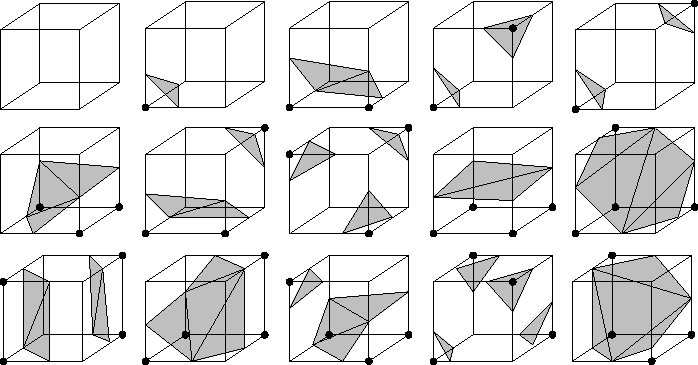
\includegraphics[width=15cm,keepaspectratio]{obr/mccase.pdf}
\caption{Unikátní konfigurace, obrázek převzat z \cite{MARCHINGCUBESCASE}}
\label{fig:mccase}
\end{figure}

Na hranách krychle se vyskytuje vrchol geometrie (trojúhelníku) v případě, kdy ohodnocení rohů krychle, které hrana sdílí, není stejné (na jednom rohu je $0$ a na druhém $1$).
Vznikne tak několik hran, na kterých leží vrcholy trojúhelníků.
Vhodným propojením vrcholů vznikne trojúhelníková síť pro jednu konfiguraci krychle.
Patnáct trojúhelníkových sítí pro patnáct unikátních konfigurací můžeme vidět na obrázku \ref{fig:mccase}.
Spojením všech trojúhelníkových sítí ze všech krychlí rozmístěných v prostoru vznikne výsledná síť.


Marching cubes algoritmus má jednu nevýhodu.
Některé konfigurace krychlí spolu nejsou kompatibilní podle \cite{MARCHINGCUBES}.
Pokud bychom nekompatibilní stavy neřešili, ve výsledné troj\-ú\-hel\-ní\-ko\-vé síti by vznikly díry.
Obslužný kód by nám zbytečně zvětšil aplikaci, a tak není algoritmus Marching cubes v této podobě v práci použit.

\subsection{Marching tetrahedra}
Marching tetrahedra algoritmus (kráčející čtyřstěn) už netrpí problémem nekompatibilních konfigurací jako Marching cubes.
Nicméně produkuje větší množství geometrie.
Stejně jako u předcházejícího algoritmu potřebujeme funkci, která rozhodne, zda daný bod leží uvnitř nebo vně objektu.
Čtyřstěn má čtyři rohy, proto je celkový počet konfigurací roven $2^4$.
Maximální počet trojúhelníků v jedné konfiguraci je $2$.
Vzhledem k těmto malým číslům si můžeme jednotlivé konfigurace vhodně uložit do konstantních dat programu.

Problém tohoto algoritmu spočívá v rozmístění čtyřstěnů v prostoru s objektem.
Pokud bychom použili čtyřstěn, který má všechny hrany stejně dlouhé, rozmístění v prostoru by nebylo úplně snadné (tak jako u krychle u předešlého algoritmu).
Algoritmus na rozmístění čtyřstěnu by nám zbytečně obsadil místo v programu.
Proto rozmístíme šest čtyřstěnů do krychle.
Tuto krychli budeme pravidelně rozmísťovat do prostoru stejně jako u algoritmu Marching cubes.
Rozmístění čtyřstěnů v krychli můžeme vidět na obrázku \ref{fig:tetraincube}.
Pro vrcholy krychle spočteme, zda leží uvnitř či vně objektu.
Poté pro všech šest čtyřstěnů vybereme z tabulky správnou trojúhelníkovou síť.

\begin{figure}[h]
\centering
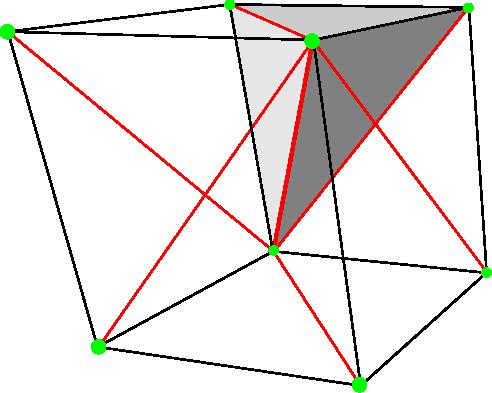
\includegraphics[width=5cm,keepaspectratio]{obr/tetra.pdf}
\caption{Rozmístění čtyřstěnů do krychle}
\label{fig:tetraincube}
\end{figure}

\subsection{Vyhlazení}

Pokud bychom u algoritmů uvedených výše umísťovali vrcholy trojúhelníků přímo doprostřed hrany na které leží, výsledná trojúhelníková síť by byla hranatá.
Hranatou troj\-ú\-hel\-ní\-ko\-vou síť můžeme vidět v levé části obrázku \ref{fig:vyhlaz}.
Vhodným posunutím vrcholů na hranách můžeme dosáhnout vyhlazení (pravá část obrázku \ref{fig:vyhlaz}.
Body na hranách můžeme posunou podle toho, jak daleko jsou konce hrany od předpokládaného povrchu.

Pokud použijeme objemovou reprezentaci (například šum), hodnota v prostoru nám určuje hustotu.
Hodnotu hustoty budeme brát v rozsahu $\langle 0,1 \rangle$.
Když hodnota hustoty na daných souřadnicích překročí hodnotu prahu $T$, nachází se v místech souřadnic těleso.
Hustotu v bodech na souřadnicích $S_a,S_b$ na koncích hrany označme $H_a,H_b$.
Zároveň platí podmínka, že právě jeden bod konce hrany leží v tělese:$(H_a \geq T \wedge H_b < T) \vee (H_a < T \wedge H_b \geq T)$.
Souřadnice vrcholu na hraně jsou dány vztahem: $(1-t)\cdot S_a + t \cdot S_b$.
Parametr $t$ je vypočítán podle vztahu: $t=\frac{T-H_a}{H_b-H_a}$.

\begin{figure}[htb]
\centering
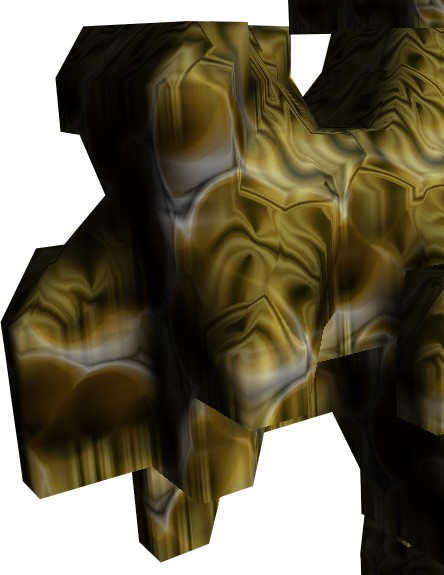
\includegraphics[width=5cm,keepaspectratio]{obr/mt_nevyhlaz.jpg}
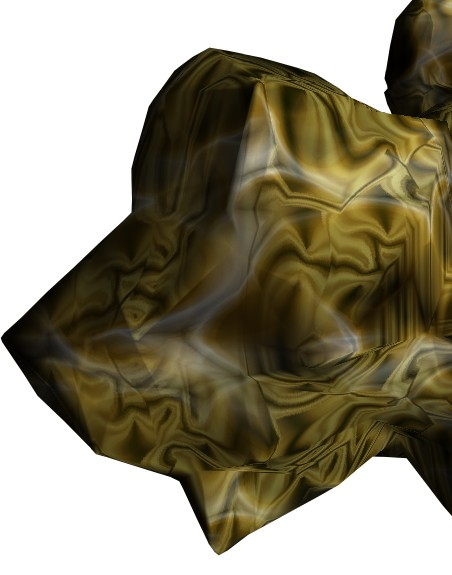
\includegraphics[width=5cm,keepaspectratio]{obr/mt_vyhlaz.jpg}
\caption{Marching tetrahedra. Vlevo: bez vyhlazení. Vpravo: s vyhlazením.}
\label{fig:vyhlaz}
\end{figure}

\subsection{Zmenšení počtu vrcholů}
Výše uvedené algoritmy produkují mnoho geometrie.
Pokud budeme data ukládat do spo\-leč\-né\-ho pole, nebudeme mít informaci o tom, který vrchol je sdílen vícero trojúhelníky.
Daný bod na hraně jedné krychle je vygenerován i jinou sousední krychlí a je uložen do společného pole několikrát.
Navíc toto způsobuje problém při výpočtu normál.
Proto je vhodné vrcholy, které jsou duplicitní uložit do pole jen jednou.
Toto lze zajistit jednoduše.
Budeme vrcholy do společného pole vkládat postupně.
Vždy porovnáme souřadnice právě vkládaného vrcholu se všemi vrcholy, které jsou již uloženy.

Toto řešení má nevýhodu a tou je rychlost.
Pro velké množství vrcholů je potřeba provést velké množství porovnání.
Proto budeme vrcholy ukládat do stromu.
Pokud budeme chtít zjistit, zda byl již daný bod uložen, stačí prohledat jen malou část stromu.
Toto algoritmus urychlí.

\subsection{Normály}
\label{subsec:normal}
Normály se v počítačové grafice používají pro stínování objektů a práci se světlem.
Můžeme si ukládat normálu ke každé plošce.
Normála je v tomto případě stejná pro všechny body plošky (polygonu).
Tímto dosáhneme jednolitého stínování.
Jednolité stínování můžeme použít pro ploché objekty jako jsou stěny, podlaha nebo například bedny.
Další možností je ukládat si normálu ke každému vrcholu polygonu.
Poté budeme osvětlení počítat pro všechny vrcholy polygonu a uvnitř osvětlení interpolovat.
Vizuálně lepší výsledky ale do\-sta\-ne\-me, pokud budeme interpolovat normály.
Pro každý bod polygonu tak budeme mít k dispozici interpolovanou normálu, kterou použijeme pro výpočet osvětlení.
Díky interpolaci normály nepotřebujeme tolik polygonů (trojúhelníků) pro reprezentaci hladkého objektu.
Výpočet normály pro vrchol, který je sdílen $k$ trojúhelníky s normálami a obsahy $\overline{n}_i,s_i, i \in \{1,\dotsc,k \}$ je dán vztahem:

\begin{equation}
\label{eq:normaly0}
n=nor \left(\sum_{i=1}^k \overline{n}_i \cdot s_i \right)
\end{equation}

Funkce $nor$ normalizuje vstupní vektor. Můžeme se obejít bez výpočtu obsahu troj\-ú\-hel\-ní\-ků a vztah \ref{eq:normaly0} zjednodušit na:

\begin{equation}
\label{eq:normaly1}
n=nor \left(\sum_{i=1}^k \overline{n}_i \right)
\end{equation}

Problém nastane, pokud jsou v objektu velmi úzké trojúhelníky.
U velmi úzkých troj\-ú\-hel\-ní\-ků je hlavní část vyhlazení normál zastoupena v malé oblasti.
Povrch objektu je sice vystínován plynule, ale z větší vzdálenosti se již tak nejeví.
V levé části obrázku \ref{fig:normaly} můžeme pozorovat hranice trojúhelníků, které sousedí s velmi úzkými trojúhelníky.
Algoritmus marching tetrahedra bohužel produkuje tyto úzké trojúhelníky pokud je zapnuto vyhlazování.
Buď budeme mít stejně velké trojúhelníky a vizuálně hladkou interpolaci normál, ale hranatý objekt nebo hladký objekt a viditelné hrany trojúhelníků.
Řešení můžeme vidět v algoritmu, který by pro daný vrchol nepočítal normály jen z trojúhelníků, které tento vrchol sdílí, ale z většího okolí.
Implementováním tohoto řešení bychom ale zbytečně zabrali místo v aplikaci.

Elegantní řešení spočívá v použití gradientu (směru růstu) trojrozměrného šumu, který jsme použili pro vygenerování geometrie, postup je blíže popsán v \cite{KASKADY}.
Normály reprezentované pomocí gradientu můžeme vidět v pravé části obrázku \ref{fig:normaly}.
Gradient trojrozměrného šumu si můžeme uložit do trojrozměrné textury a využít jej také pro počítání kolizí.
Výpočet gradientu v bodě o souřadnicích $I=(i_1,i_2,i_3)$ získáme pomocí vztahu:
\begin{equation}
\label{eq:norgrad}
g=(h(I+x)-h(I-x),h(I+y)-h(I-y),h(I+z)-h(I-z))
\end{equation}
Ve vztahu \ref{eq:norgrad} reprezentuje $x$ respektive $y$ respektive $z$ trojici $(1,0,0)$ respektive $(0,1,0)$ respektive $(0,0,1)$.
Funkce $h(I)$ vrací hodnotu šumu na souřadnicích I.
Výpočet normály z gradientu je jednoduchý stačí gradient znormalizovat.


\begin{figure}[h]
\centering
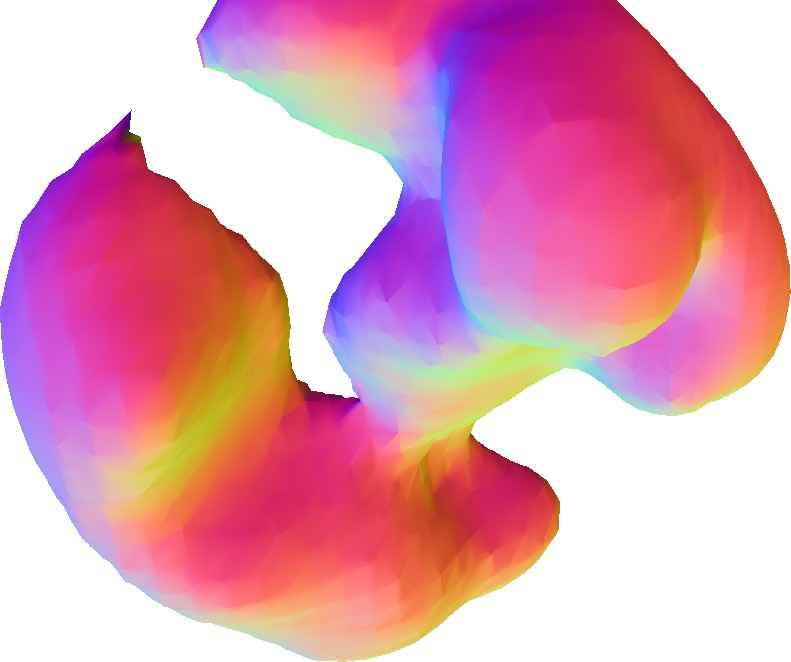
\includegraphics[width=7.5cm,keepaspectratio]{obr/normalsum.jpg}
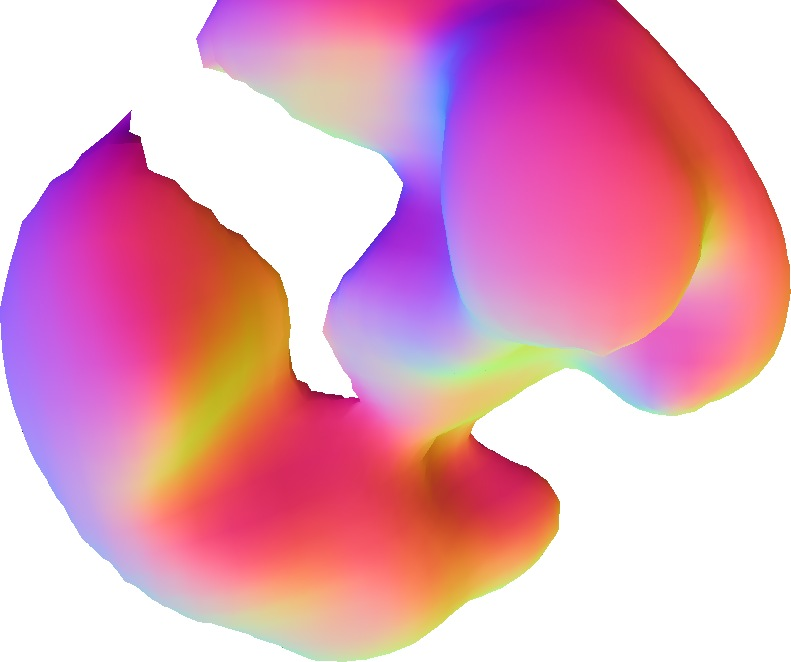
\includegraphics[width=7.5cm,keepaspectratio]{obr/normalgradient.jpg}
\caption{Zobrazení normál. Vlevo: normály pro vrcholy trojúhelníků. Vpravo: normály reprezentované gradientem.}
\label{fig:normaly}
\end{figure}



